\documentclass[arhiv]{../izpit}
\usepackage{fouriernc}
\usepackage{tikz}
\usepackage{censor}
\usepackage{paralist}

\begin{document}

\izpit{Programiranje I: 3\ izpit}{4.\ mali srpan 2014}{
  Čas reševanja je 150 minut.
  Doseženih 100 točk šteje za maksimalno oceno.
  Veliko uspeha!
}

%%%%%%%%%%%%%%%%%%%%%%%%%%%%%%%%%%%%%%%%%%%%%%%%%%%%%%%%%%%%%%%%%%%%%%
\naloga[Vojska Republike Banana, 10 + 10 + 10 točk]
Tudi v Republiki Banana so vojaki urejeni hierarhično, tako kot povsod drugod. Vsakdo razen vrhovnega poveljnika oboroženih banan ima natanko enega nadrejenega. Vsak vojak lahko po\-vel\-ju\-je največ dvema podrejenima (levemu in desnemu). Primer takšne vojaške hierarhije:
$$
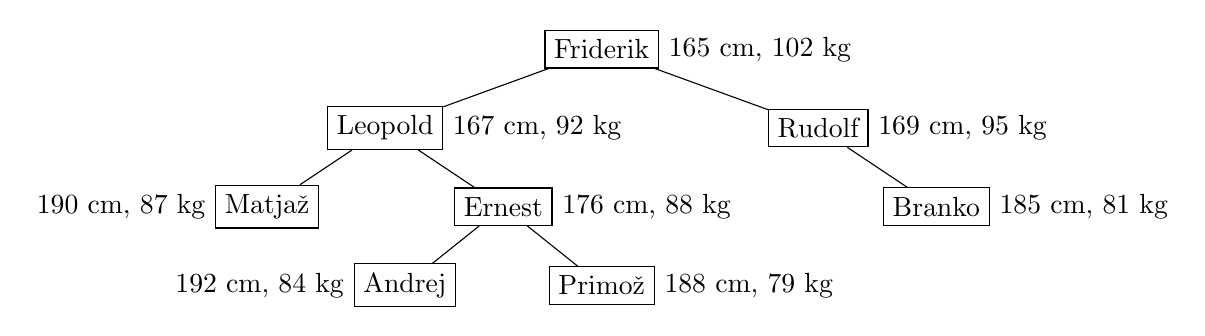
\begin{tikzpicture}[level distance=1cm,
    level 1/.style={sibling distance=5.5cm},
    level 2/.style={sibling distance=3cm},
    level 3/.style={sibling distance=2.5cm}
    ]
    \node[rectangle, draw, label=0:{165 cm, 102 kg}] (d) {Friderik}
      child {node[rectangle, draw, label=0:{167 cm, 92 kg}] {Leopold}
        child {node[rectangle, draw, label=180:{190 cm, 87 kg}] {Matjaž}}
        child {node[rectangle, draw, label=0:{176 cm, 88 kg}] {Ernest}
          child {node[rectangle, draw, label=180:{192 cm, 84 kg}] {Andrej}}
          child {node[rectangle, draw, label=0:{188 cm, 79 kg}] {Primož}}
        }
      }
      child {node[rectangle, draw, label=0:{169 cm, 95 kg}] {Rudolf}
        child[missing] {}
        child {node[rectangle, draw, label=0:{185 cm, 81 kg}] {Branko}}
      };
  \end{tikzpicture}
$$
Raziskava Ministrstva za napad je razkrila, da vojska poje ogromno količino banan. Njihova skupna kalorična vrednost bi morala zadoščati za dvakrat večjo armado. Na ministrstvu zaradi teh dejstev domnevajo, da so nekateri vojaki predebeli. Ker bi radi zadevi prišli do dna, so ključne podatke o vojakih shranili v podatkovno strukturo \texttt{Drevo}, ki je že implementirana. V vozliščih drevesa so shranjeni naslednji podatki o vojakih: višina v cm (atribut \texttt{visina}), masa v kg (atribut \texttt{masa}) in ime vojaka (atribut \texttt{ime}).

\podnaloga[10 točk]
Sestavite funkcijo \texttt{naloga1a(self)}, ki vsakemu vozlišču v drevesu pripne še atribut \texttt{itm}, pri čemer naj bo rezultat zaokrožen na dve decimalki. (Nasvet: Za zaokroževanje uporabite funkcijo \texttt{round(x, n)}.) Funkcija \texttt{naloga1a} naj ne vrača ničesar. Indeks telesne mase (s kratico ITM) se izračuna po formuli
$$\mathit{ITM} = \frac{m}{v^2},$$
kjer je $m$ masa v kg, $v$ pa višina v m. Vojak Branko (glejte zgornji primer) ima torej
$$\mathit{ITM} = \frac{81}{1,85^2} \approx 23,\!67.$$

\podnaloga[10 točk]
Z ministrstva je prišla direktiva, da je treba najdebelejše tri vojake v poduk ostalim izstradati do smrti. Vrhovni poveljnik zahteva, da napišite funkcijo \texttt{naloga1b(self)}, ki vrne seznam treh najdebelejših vojakov (oz.\ manj, če ima drevo manj kot 3 vozlišča). Vsak vojak v seznamu naj bo predstavljen s parom: prva kompotenta naj bo ime vojaka, druga komponenta pa njegov ITM. Seznam naj bo urejen padajoče glede na ITM. Primer (če \texttt{d} ustreza zgornji sliki):
%
\begin{verbatim}
>>> d.naloga1b()
[('Friderik', 37.47), ('Rudolf', 33.26), ('Leopold', 32.99)]
\end{verbatim}
%
Pri tej in naslednji podnalogi lahko predpostavite, da nobena dva vojaka nimata enakega ITM.

\podnaloga[10 točk]
Ko je vrhovni poveljnik videl, da je tudi on sam na seznamu, je ``zašvical ful''. Zahteva, da napišite novo funkcijo \texttt{naloga1c(self)}, ki bo najdebelejše tri poiskala samo med vojaki, ki \emph{niso} častniki. \emph{Častniki} so natanko tisti, ki imajo pod seboj vsaj enega podrejenega. Primer:
%
\begin{verbatim}
>>> d.naloga1c()
[('Matjaž', 24.1), ('Branko', 23.67), ('Andrej', 22.79)]
\end{verbatim}
(Za ``neprijetnost'' iz druge podnaloge na ministrstvu ne smejo nikoli izvedeti, sicer \ldots)

%%%%%%%%%%%%%%%%%%%%%%%%%%%%%%%%%%%%%%%%%%%%%%%%%%%%%%%%%%%%%%%%%%%%%%
\naloga[Gregorijanski koledar, 20 + 15 točk]

Leta 1582 je takratni papež Gregor XIII.\ uvedel gregorijanski koledar. Namen reforme je bil,
da se povprečno dolžino koledarskega leta bolj približa dejanski dolžini sončevega leta. 

Oba koledarja poznata navadna leta, ki imajo 365, in prestopna leta, ki imajo 366 dni. V na\-vad\-nem
letu ima mesec februar 28 dni, v prestopnem letu pa še en dan več (29.\ februar). Razlika med
obema koledarjema je le to, kako se določi prestopno leto. Pri \emph{julijanskem} koledarju so
prestopna vsa leta, ki so deljiva s 4. Pri \emph{gregorijanskem} koledarju je pravilo malo bolj
zapleteno: Leto je prestopno, če je deljivo s 4 in ni deljivo s 100 ali pa če je deljivo s 400.
Leta 1600, 1700, 1800, 1900, 2000, 2100, 2200, 2300 in 2400 so vsa prestopna v \emph{julijanskem}
koledarju. V \emph{gregorijanskem} koledarju pa so med tistimi iz gornjega seznama prestopna le
1600, 2000 in 2400.

Pri starem julijanskem koledarju je bila povprečna dolžina leta $365,\!25$ dni. Pri gregorijanskem
koledarju je popvrečna dolžina leta $365,\!2425$ dni. Glede na to, da je dolžina sončevega leta
približno  $365,\!24219$ dni, je očitno, da je gregorijanski koledar velika izboljšava.

Del papeževe reforme je bilo tudi to, da smo pri prehodu na nov koledar nekaj dni izpustili, da bi
izničili učinek 1500 let trajajoče zablode. Papež je odredil, da bo 4.\ oktobru 1582 (po julijansko)
sledil 15.\ oktober 1582 (po gregorijansko). Mnoge nekatoliške države so še dolgo po reformi uporabljale
julijanski koledar. V Združenem kraljestvu Velike Britanije in Severne Irske so na greogrijanski koledar
prešli po 2.\ septembru 1752 (ki mu je sledil 14.\ september 1752). V Evropi je kot zadnja na gregorijanski koledar
prešla Grčija, kjer so na novi koledar prešli šele po 15. februarju 1923 (ki mi je sledil 1. marec 1923).

\podnaloga[20 točk]
Sestavite funkciji \texttt{jul\_jutri(d, m, l)} in \texttt{greg\_jutri(d, m, l)}. Obe funkciji kot
vhodni podatek dobita datum, podan z argumenti \texttt{d} (dan), \texttt{m} (mesec) in \texttt{l} (leto).
Funkciji naj
vrneta datum naslednjega dne in sicer kot nabor \texttt{(d, m, l)}. Prva funkcija naj upošteva
julijanski koledar, druga pa gregorijanskega. Primer:
%
\begin{verbatim}
>>> jul_jutri(28, 2, 1900)
(29, 2, 1900)
>>> greg_jutri(28, 2, 1900)
(1, 3, 1900)
\end{verbatim}
%
Predpostavite, da bosta funkciji vedno dobili veljavne vhodne podatke.
%
\podnaloga[15 točk] Sestavite funkcijo \texttt{jul2greg(d, m, l)}, ki naj datum v julijanskem koledarju pretvori v datum v
gregorijanskem koledarju. Predpostavite, da bodo vsi vhodni podatki veljavni in kasnejši kot 4.\ oktober 1582.
Primer:
%
\begin{verbatim}
>>> jul2greg(16, 2, 1923)
(1, 3, 1923)
\end{verbatim}
%
Nasvet: Funkcijo lahko sestavite na primer tako, da si naredite dva nabora in sicer:
\begin{verbatim}
jul = (5, 10, 1582)
greg = (15, 10, 1582)
\end{verbatim}
Nato pa znotraj zanke na komponentah naborov \texttt{jul} in \texttt{greg} uporabljate funkciji \texttt{jul\_jutri} in \texttt{greg\_jutri}, dokler \ldots

%%%%%%%%%%%%%%%%%%%%%%%%%%%%%%%%%%%%%%%%%%%%%%%%%%%%%%%%%%%%%%%%%%%%%%
\naloga[Sedla, 25 točk]

Za element realne matrike bomo rekli, da je \emph{sedlo}, če je večji ali enak vsem ostalim v isti vrstici ter manjši ali enak vsem ostalim v istem stolpcu (torej je maksimum v svoji vrstici in minimum v svojem stolpcu).

Matrika lahko vsebuje več sedel, lahko pa tudi nobenega. Na primer matrika
$$\begin{bmatrix} 1 & 2 & 3 \\ 4 & 5 & 6 \\ 1 & 2 & 3 \end{bmatrix}$$
ima dve sedli in sicer sta to element z indeksoma $(1, 3)$ in element z indeksoma $(3, 3)$. (Prvi indeks je indeks vrstice, drugi pa indeks stolpca.)

V \emph{Mathematici} sestavite funkcijo \texttt{sedla[a\_]}, ki poišče vsa sedla matrike \texttt{a} in vrne urejen sez\-nam parov indeksov. Primer:
%
\begin{verbatim}
In[1]:= sedla[{{1, 2, 3}, {4, 5, 6}, {1, 2, 3}}]
Out[1]= {{1, 3}, {3, 3}}
\end{verbatim}
%
Lahko si naredite poljubno mnogo pomožnih funkcij.

%%%%%%%%%%%%%%%%%%%%%%%%%%%%%%%%%%%%%%%%%%%%%%%%%%%%%%%%%%%%%%%%%%%%%%
\naloga[Hiperkocke, 30 točk]

V \emph{Mathematici} sestavite funkcijo \texttt{hiperkocka[n\_]}, ki izriše sliko $n$-dimenzionalne hiperkocke. To je graf z $2^n$ vozlišči, ki so označena s števili od 0 do $2^n-1$. Vozlišča naj bodo ekvidistančno razporejena po enotski krožnici. Skrajno desno vozlišče na krožnici naj ima oznako 0. V nasprotni smeri urinega kazalca pa naj sledijo vozlišča 1, 2, 3, \ldots

Med vozliščema z oznakama $i$ in $j$ je povezava, če je Hammingova razdalja med njunima binarnima zapisoma natanko 1.
Na primer, binarni zapis števila 9 je 1001, binarni zapis števila 11 pa je 1011. \emph{Hammingova razdalja} med dvema nizoma je število mest, na katerih se ta dva niza razlikujeta. Ker se niza \texttt{1001} in \texttt{1011} razlikujeta le na enem mestu (3.\ znak z leve), je Hammingova razdalja med njima 1.

\begin{center}
\begin{tabular}{c@{\hspace{1.5cm}}c@{\hspace{1.5cm}}c}
 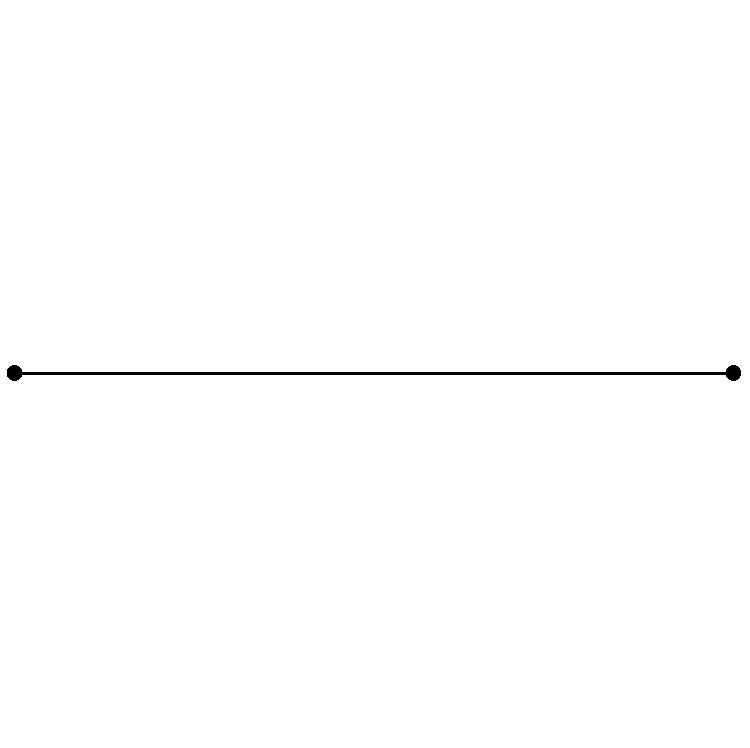
\includegraphics[width=4cm]{hiperkocka1.pdf}&
 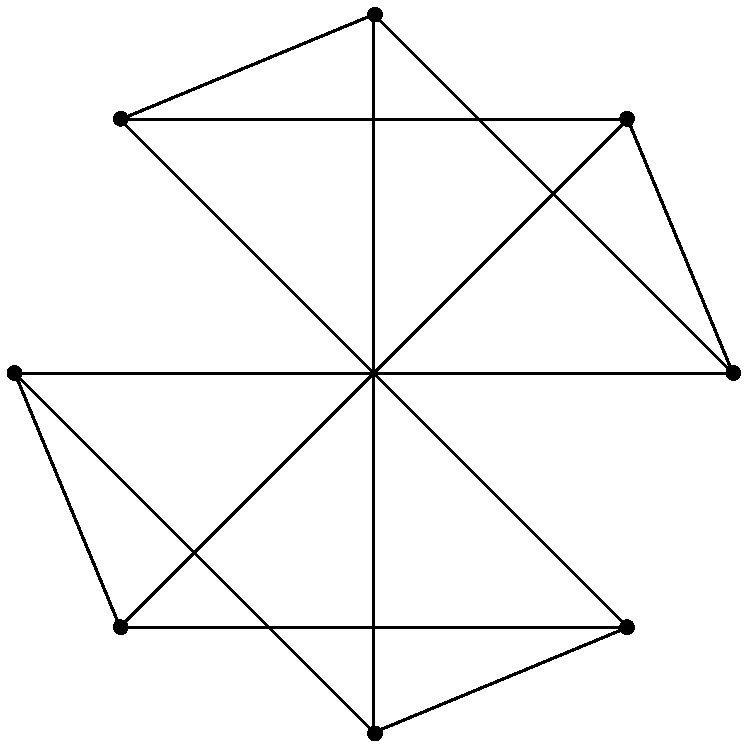
\includegraphics[width=4cm]{hiperkocka3.pdf}&
 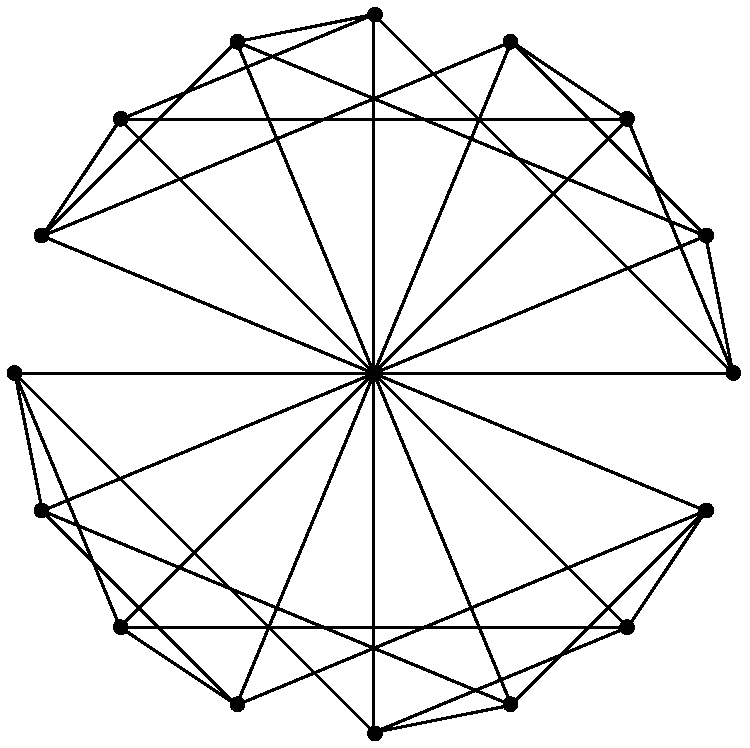
\includegraphics[width=4cm]{hiperkocka4.pdf}\\
  \texttt{hiperkocka[1]} &
  \texttt{hiperkocka[3]} &
  \texttt{hiperkocka[4]}
\end{tabular}
\end{center}
%
Nasvet 1: Hammingova razdalja med binarnima zapisoma števil \texttt{i} in \texttt{j} je ravno število enic v binarnem zapisu števila \texttt{BitXor[i, j]}.

\vspace{\baselineskip}
\noindent
Nasvet 2: Seznam števk števila \texttt{n} zapisanega v bazi \texttt{b} nam da funkcija \texttt{IntegerDigits[n, b]}.
% naloga3[n_] := Graphics[{
%    Table[Line[{{-k, 0}, {-k + 1, 0}}], {k, 1, n, 2}],
%    Table[Line[{{0, -k}, {0, -k + 1}}], {k, 2, n, 2}],
%    Table[Line[{{-k, 0}, {-k, -k}, {0, -k}}], {k, 1, n}]}]

\end{document}

